\chapter{Part IV(d) - Instruction Level Parallelism - Scheduling}
\section{Dynamic Scheduling and Out-of-Order Execution}
\label{sec:dynsched}

Modern processors often employ \textbf{dynamic scheduling} to exploit more instruction-level parallelism
(ILP). Instead of strictly following the program’s original instruction order
(\emph{in-order} execution), the processor can:

\begin{itemize}
  \item \textbf{Fetch and decode} instructions as early as possible, even if previous
        instructions have not completed.
  \item \textbf{Reorder} instruction execution to avoid idle functional units when
        long-latency instructions (e.g., divides) are in progress.
  \item \textbf{Ensure correctness} by respecting true data dependencies and properly
        writing results back in program order (via a \emph{Reorder Buffer (ROB)}).
\end{itemize}

\subsection{Motivating Example}
Consider the following sequence of floating-point operations:
\begin{verbatim}
  divd  $f0, $f2, $f4    # Long-latency division
  addd  $f10, $f0, $f8   # Depends on divd's result
  subd  $f12, $f8, $f14  # Independent of divd's result
\end{verbatim}

\begin{itemize}
  \item In a strict in-order pipeline, the \texttt{subd} could be stalled until
        \texttt{divd} completes its execution (because \texttt{addd} is waiting
        on \$f0).
  \item With dynamic scheduling, the processor can reorder
        \texttt{subd} before \texttt{addd} as soon as it identifies that
        \texttt{subd} does \emph{not} depend on \texttt{divd}.
  \item This reordering utilizes available resources without violating correctness.
\end{itemize}

\subsection{Breaking the Rigidity of Basic Pipelines}
In a standard five-stage pipeline (Fetch, Decode, Execute, Memory, Writeback),
stalls are common when earlier instructions hold resources or have unresolved
data dependencies. Dynamic scheduling mitigates these stalls by:
\begin{enumerate}
  \item \textbf{Continuing to fetch and decode} new instructions (even if some are
        stalled in execution).
  \item \textbf{Deferring writeback} until resources become available or dependencies
        are resolved, using dedicated hardware structures (e.g., reservation
        stations, reorder buffers).
  \item \textbf{Allowing out-of-order completion}: instructions finish as soon as they
        can, but their results are committed in-order to preserve program semantics.
\end{enumerate}

\subsection{Dynamically Scheduled Processor Overview}
A typical dynamically scheduled CPU integrates:
\begin{itemize}
  \item \textbf{Fetch/Decode} units that feed instruction information into
        \emph{reservation stations} (RS).
  \item Multiple functional units (ALU, FPU, Memory pipelines) operating in
        parallel.
  \item A \textbf{Reorder Buffer (ROB)} to track instruction completion and to
        ensure in-order retirement (commit) of results.
  \item \textbf{Forwarding paths} to provide operands directly to waiting instructions
        without requiring all results to be written back to the register file first.
\end{itemize}

By decoupling instruction fetch/decode from their actual execution, a
\textbf{dynamically scheduled processor} allows more effective use of hardware
resources and improves overall performance, particularly for workloads with
long-latency operations or frequent stalls in in-order pipelines.
\subsection{Reservation Stations}

Reservation stations are hardware queues that temporarily hold instructions before they are sent to an execution unit. They are a key component in enabling \textbf{out-of-order execution} within a processor. This mechanism allows the CPU to execute instructions as soon as their necessary resources are available, rather than strictly adhering to the program's original order.

\subsubsection{How Reservation Stations Work}

Reservation stations facilitate several critical functions in the CPU:

\begin{enumerate}
    \item \textbf{Check Operand Availability:}
    They verify that all input operands required by an instruction have been computed and are available, either in the register file or through bypassing from another execution unit.

    \item \textbf{Prevent Structural Hazards:}
    They ensure that the targeted execution unit is free and ready to accept a new operation, thereby avoiding conflicts over shared functional units.

    \item \textbf{Enable Dynamic Scheduling:}
    They allow instructions to be dispatched to available execution units as soon as both their operands and the necessary functional resources are ready, rather than waiting for earlier instructions to complete.
\end{enumerate}

\subsubsection{Components of a Reservation Station}

Each entry within a reservation station typically contains the following elements:

\begin{itemize}
    \item \textit{Operation Code} (e.g., \texttt{add}, \texttt{sub}, \texttt{mul}): Specifies the operation to be performed.
    \item \textit{Operands or Tags}: Contains the actual operands needed for the operation or tags that reference future instructions responsible for producing those operands.
    \item \textit{Status Bits}: Indicate whether the operands are ready and whether an appropriate execution unit has been reserved.
\end{itemize}

\subsubsection{Execution Process}

\begin{enumerate}
    \item \textbf{Issuing Instructions:} When an instruction enters a reservation station, it waits until both its operands are available and the required execution unit is free.
    \item \textbf{Executing Instructions:} Once these conditions are met, the reservation station issues the instruction to the execution unit.
    \item \textbf{Broadcasting Results:} After execution, the result is forwarded to all reservation stations that are waiting for that particular value, updating their entries to reflect that the operand is now valid.
\end{enumerate}

\begin{center}
    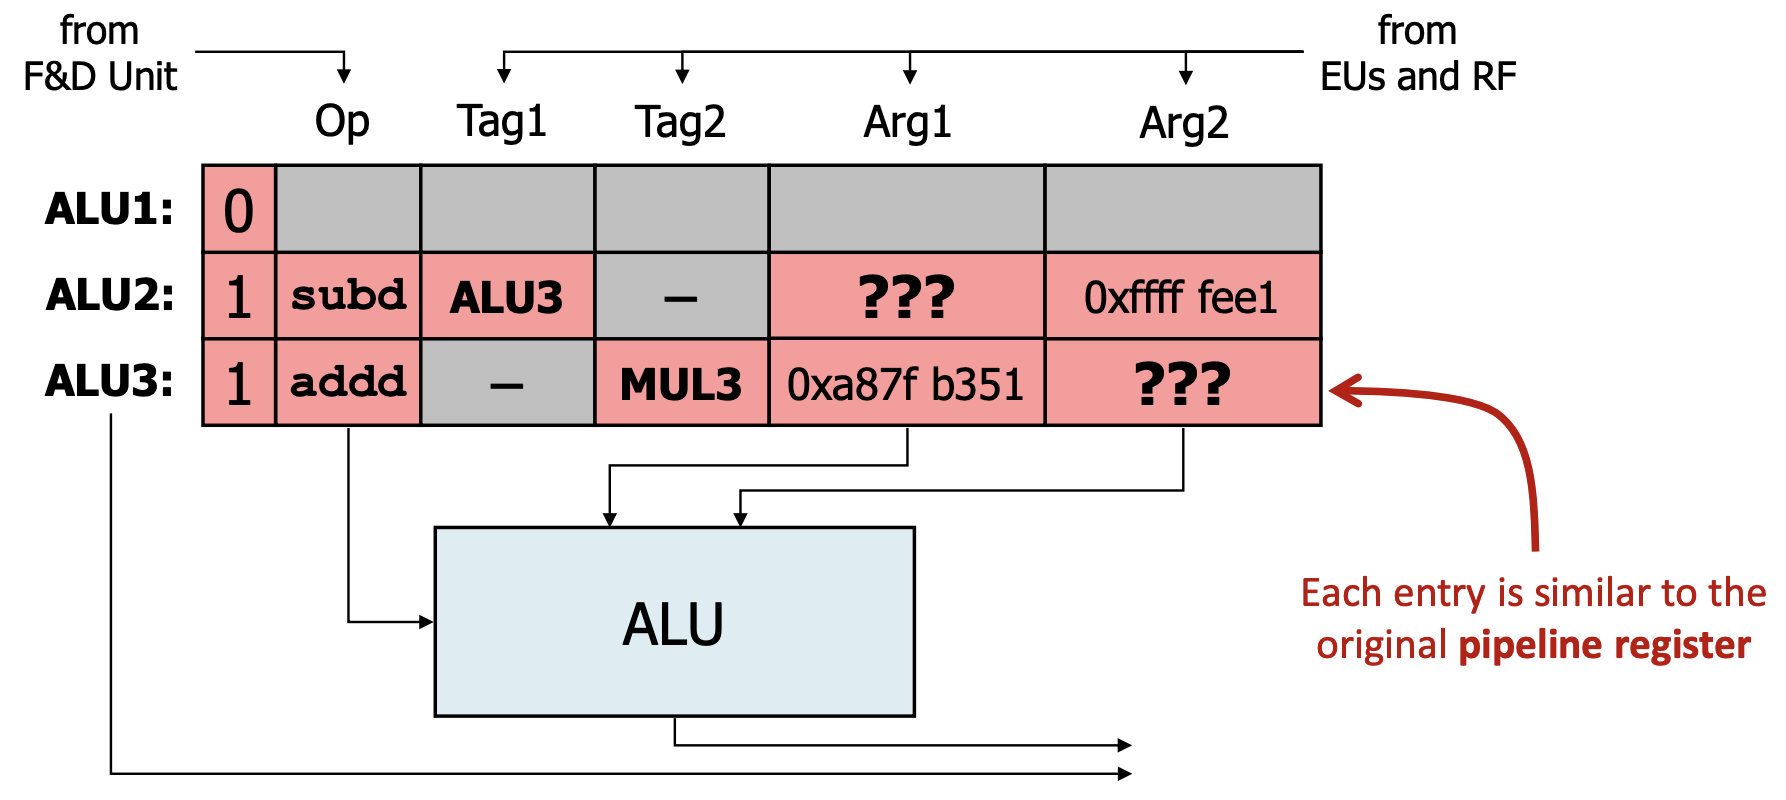
\includegraphics[width=0.65\textwidth]{chapters/chapter4d/images/reservation_table.png}
\end{center}

\subsubsection{Analogy: Kitchen Order Management}

Think of reservation stations as a \textbf{kitchen's order management system} in a restaurant:

\begin{itemize}
    \item \textbf{Orders as Instructions:} Each customer's order is an instruction that needs to be prepared.
    \item \textbf{Ingredients as Operands:} The ingredients required for each dish represent the operands. An order can only be prepared if all necessary ingredients are available.
    \item \textbf{Chefs as Execution Units:} The chefs are the execution units that prepare the dishes.
\end{itemize}

\textbf{Process Flow:}
\begin{enumerate}
    \item \textbf{Taking Orders:} Orders are placed in the reservation station (waiting area) as they come in.
    \item \textbf{Checking Ingredients:} The system verifies that all ingredients for an order are available.
    \item \textbf{Assigning to Chefs:} If ingredients are ready and a chef is available, the order is handed off to the chef for preparation.
    \item \textbf{Updating Availability:} Once a dish is prepared, the result is available to fulfill other orders that might depend on it.
\end{enumerate}

\subsubsection{Summary}
Reservation stations decouple the dispatching of instructions from the availability of their operands and the execution units. By doing so, they enhance the processor's ability to execute instructions out of order, thereby improving overall performance and efficiency.

\subsection{Register Renaming and Data Dependencies}
Register renaming is a technique used to eliminate \textbf{Write-After-Write (WAW)} and \textbf{Write-After-Read (WAR)} dependencies, collectively referred to as \textit{name dependencies}. These dependencies occur because registers are reused across multiple instructions, despite the absence of actual data flow between them.

\subsubsection{Pipeline Hazards and Dependency Types}

Pipeline execution is prone to the following dependencies:
\begin{itemize}
    \item \textbf{Read-After-Write (RAW):} True data dependence, where an instruction requires the output of a previous one.
    \item \textbf{Write-After-Write (WAW):} Name dependence, resolved by renaming.
    \item \textbf{Write-After-Read (WAR):} Name dependence, resolved by renaming.
\end{itemize}

In dynamic pipelines, out-of-order execution can introduce hazards like WAW and WAR. Renaming ensures correctness by maintaining unique register identifiers, enabling both in-order and out-of-order pipelines to avoid conflicts.

\subsubsection{Example}

Consider the following instructions:\\
\begin{minipage}[t]{0.45\textwidth}
    \begin{verbatim}
        divd  $f0, $f1, $f2
        addd  $f3, $f0, $f4
        subd  $f4, $f5, $f6
        adddi $f0, $f5, 10
    \end{verbatim}
    - \texttt{addd} has a \textbf{RAW} dependence on \texttt{divd}. \\
    - \texttt{subd} has a \textbf{WAR} dependence on \texttt{addd}. \\
    - \texttt{adddi} has a \textbf{WAW} dependence on \texttt{divd}. \\
\end{minipage}
\hfill
\vline
\hfill
\begin{minipage}[t]{0.45\textwidth}
    By renaming, these dependencies are resolved:
    \begin{verbatim}
        divd  $f0, $f1, $f2
        addd  $f3, $f0, $f4
        subd  $f30, $f5, $f6
        adddi $f29, $f30, 10
    \end{verbatim}
\end{minipage} \\ \vspace{10px}
\textbf{This ensures the pipeline executes efficiently without conflicts, improving instruction throughput.}

\newpage
\section{Dynamically Scheduled Processor}
A \emph{dynamically scheduled processor} uses hardware mechanisms to exploit
\emph{out-of-order} execution, allowing instructions to proceed as soon as
their operands become available. This contrasts with a strictly pipelined MIPS
design, where all instructions flow in \emph{order} through the five pipeline
stages (F, D, E, M, W). By dynamically scheduling instructions, the
processor can reduce stalls and more effectively utilize hardware resources.

\begin{center}
    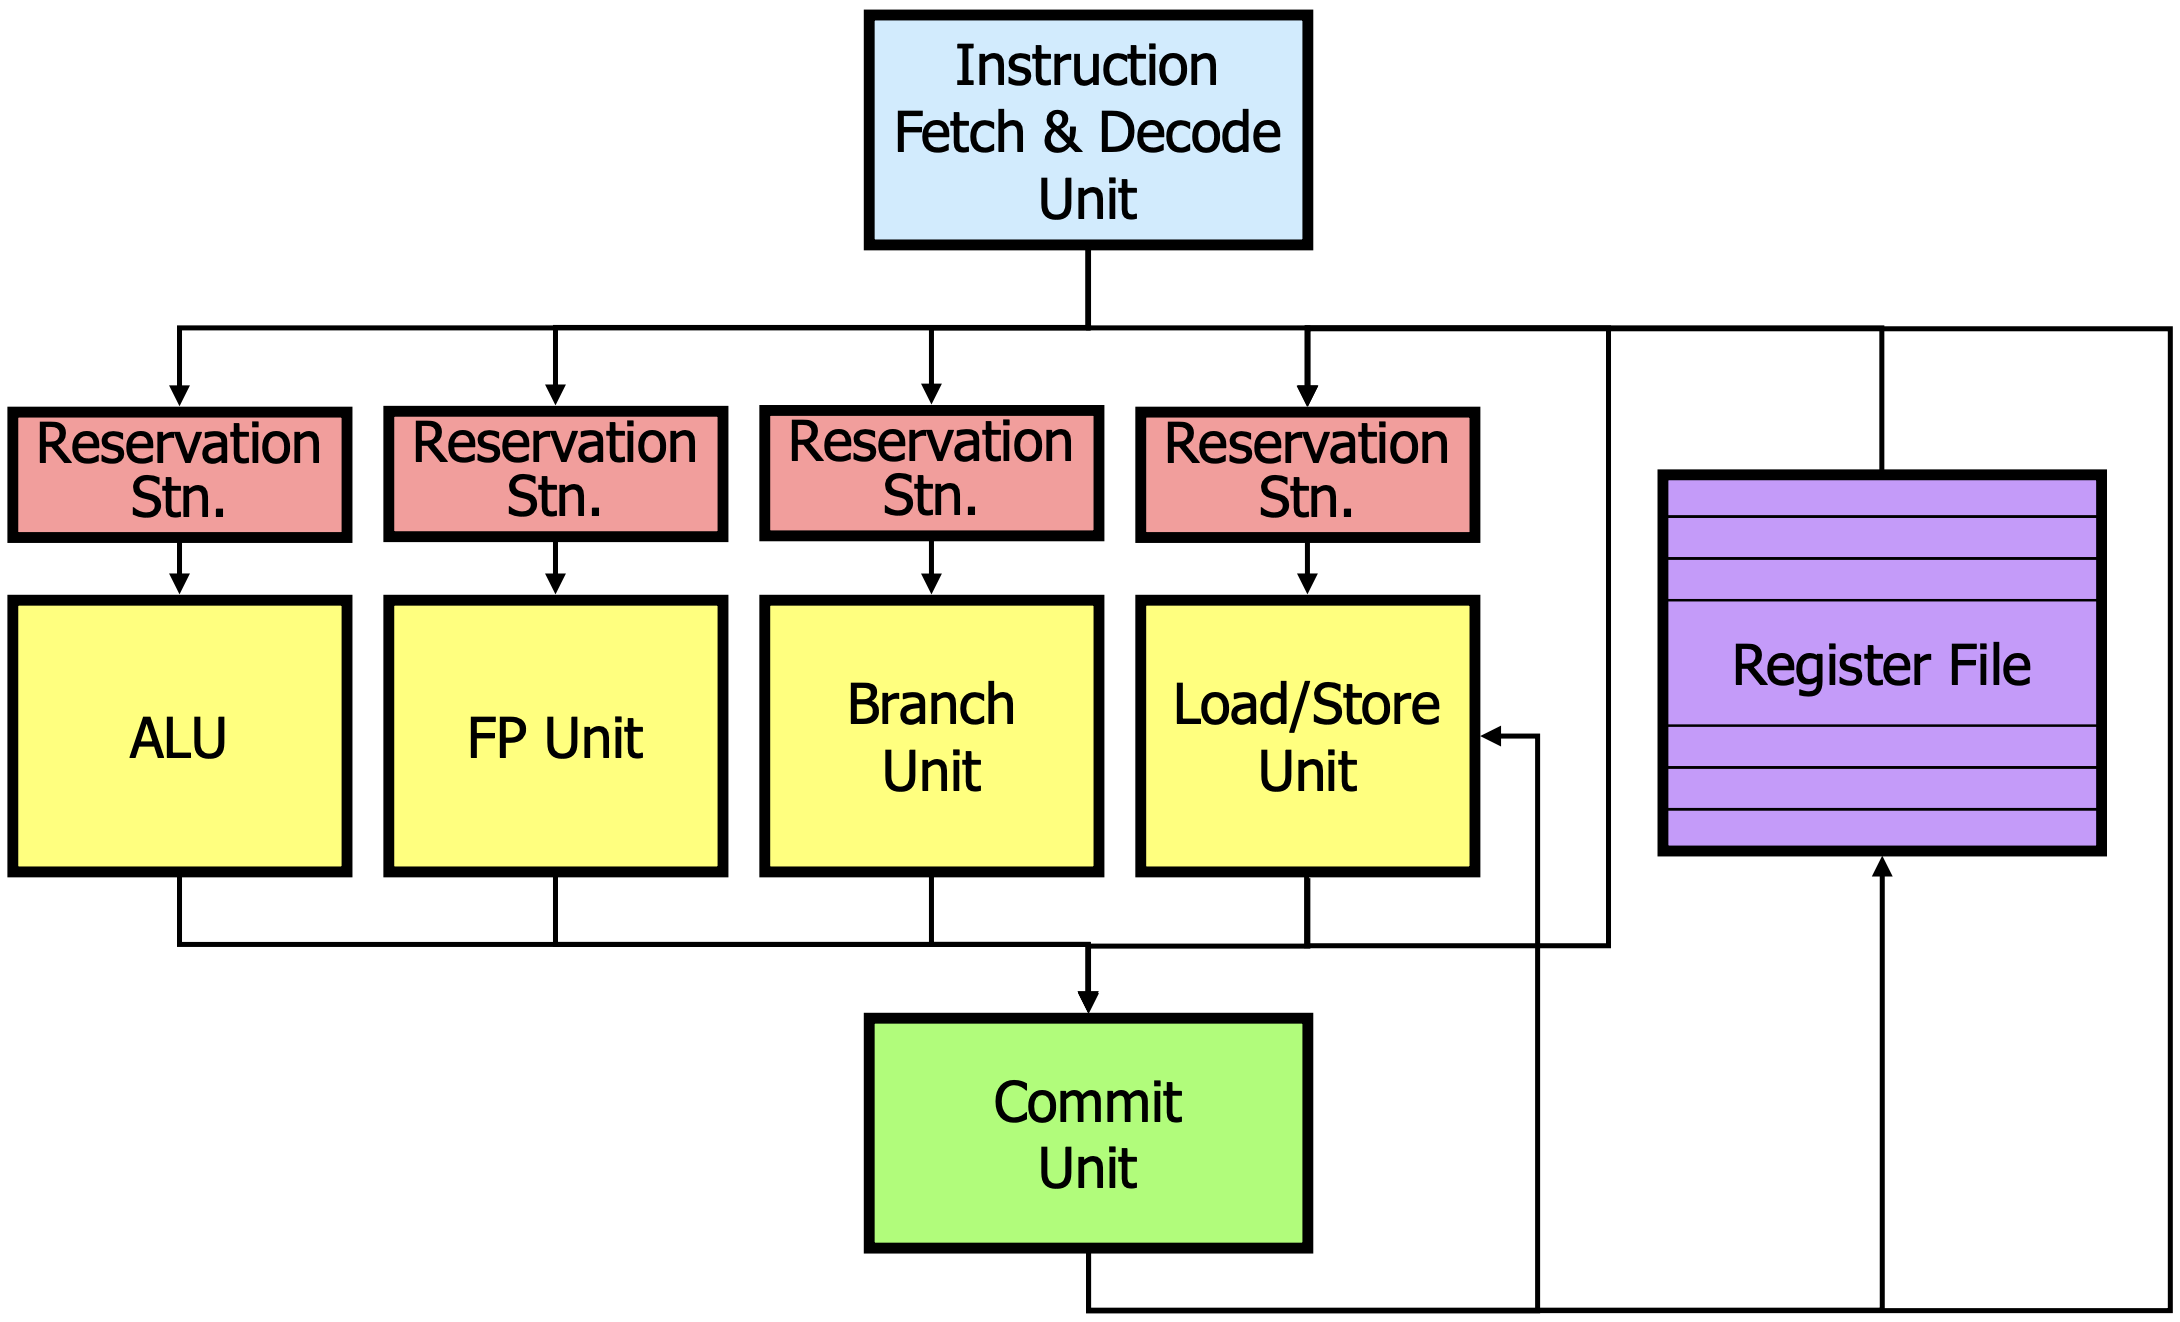
\includegraphics[width=0.65\textwidth]{chapters/chapter4d/images/complete.png}
\end{center}
\begin{itemize}
  \item[-] \textbf{Instruction Fetch \& Decode Unit:}
    Fetches and decodes instructions, dispatching them to the appropriate
    \emph{reservation stations} once the instruction type is identified.

  \item[-] \textbf{Reservation Stations:}
    Buffers that hold instructions waiting for the required operands or
    execution unit to become available. Each functional unit (e.g., ALU,
    floating-point, branch, or load/store) typically has its own set of
    reservation stations.

  \item[-] \textbf{ALU, FP Unit, Branch Unit, Load/Store Unit:}
    Execution units where instructions are actually carried out. The Load/Store
    Unit also manages memory operations. Because these units operate in parallel,
    multiple independent instructions can be serviced simultaneously.

  \item[-] \textbf{Register File:}
    Stores the architectural registers. Instructions read from and write to
    this file (potentially out of program order), but the final states are
    committed in order, preserving correct program semantics.

  \item[-] \textbf{Commit Unit:}
    Also referred to as the \emph{retirement} or \emph{write-back stage}. It
    ensures that the processor's \emph{architectural state} is updated in the
    correct program order, even though internal execution may be out of order.
\end{itemize}

\subsubsection*{Example Execution}
Suppose we have the following sequence of instructions:
\[
\begin{aligned}
&I1: \text{R1} \leftarrow \text{R2} + \text{R3}\\
&I2: \text{R4} \leftarrow \text{R1} \times \text{R5}\\
&I3: \text{R6} \leftarrow \text{R7} + \text{R8}
\end{aligned}
\]
In a strictly pipelined MIPS processor, \(\text{I2}\) would have to stall
while waiting for \(\text{R1}\) (produced by \(\text{I1}\)) to be written back.
However, a dynamically scheduled processor can place \(\text{I2}\) into a
reservation station, and simultaneously issue \(\text{I3}\) to the ALU,
because \(\text{I3}\) does not depend on \(\text{I1}\) or \(\text{I2}\).
This allows overlapping execution and reduced idle cycles.
\newpage
\subsection{Precise vs.\ Imprecise Exceptions}
Exceptions occur when the processor encounters an event requiring special handling (e.g., page fault, unsupported instruction).
They can be categorized as \emph{precise} or \emph{imprecise} based on whether the exact instruction that caused the exception---and the architectural state associated with that point in the instruction stream---can be precisely identified.

\begin{itemize}
  \item \textbf{Precise Exceptions}
  \begin{itemize}
    \item The processor enforces an in-order view of instruction completion at the point of the exception.
    \item This implies that all instructions before the faulting instruction have completed, and none of the subsequent instructions have begun or altered the architectural state.
    \item Reordering or out-of-order execution may still happen internally, but when an exception occurs, the processor ``commits'' instructions in a way that appears strictly in-order.
    \item This behavior simplifies error handling, as the operating system (OS) or exception handler knows exactly where the problem occurred and which instructions completed.
  \end{itemize}
  \item \textbf{Imprecise Exceptions}
  \begin{itemize}
    \item Out-of-order execution becomes visible to the user (or OS), meaning the faulting instruction might not be clearly identified at the time of the exception.
    \item The OS or programmer must assume that instructions have partially or fully executed in a different order than expected.
    \item Correcting the architectural state becomes more complex; the system may need to re-execute an entire subroutine to ensure correctness.
    \item Modern architectures generally avoid imprecise exceptions because of these complexities (especially for critical features such as virtual memory or I/O).
  \end{itemize}
\end{itemize}

\subsubsection{Out-of-Order Commitment and Exceptions}
Dynamic (out-of-order) execution complicates exception handling because the processor may complete some instructions after the faulting instruction if it issued them early. In a precise exception model, the hardware automatically rolls back or defers the effects of later instructions so that:
%
\begin{enumerate}
  \item Everything before the faulting instruction is guaranteed to have completed.
  \item No instructions after the faulting instruction have committed any state.
\end{enumerate}

This exact commitment model allows the exception handler to identify the precise location of the fault. When exceptions are imprecise, the program may need to be restarted from an earlier point to restore correct state, making it challenging for both the hardware and software to manage.

\newpage
\subsection{Reordering Instructions at Writeback}
A \emph{reorder buffer} (ROB) is used in out-of-order processors to maintain correct program order when writing back results to the architectural register file and memory. While instructions may execute in parallel or out of order, the ROB ensures that their visible effects (writes to registers/memory) occur in the original program order. This mechanism preserves the logical behavior of the program while also taking advantage of pipeline parallelism.
\begin{center}
    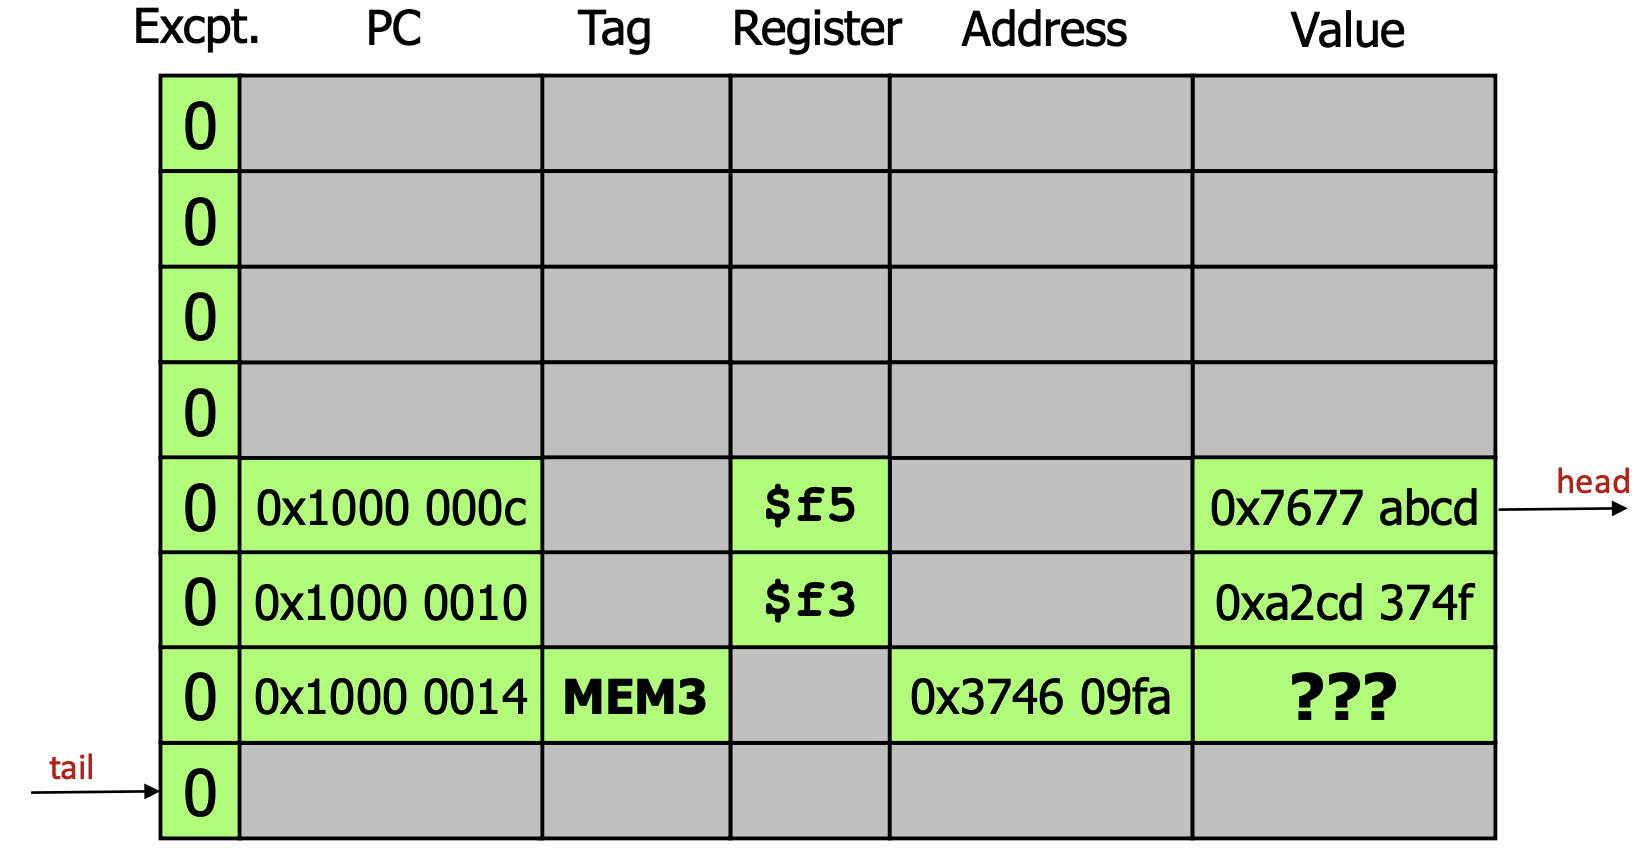
\includegraphics[width=0.65\textwidth]{chapters/chapter4d/images/rob.png}
\end{center}
\subsubsection{High-Level Overview.}
\begin{itemize}
  \item \textbf{Out-of-Order Execution:} After fetching and decoding, instructions are dispatched to execution units as soon as their operands become available. This enables the processor to exploit instruction-level parallelism.
  \item \textbf{Reorder Buffer (ROB):} Each fetched instruction is allocated an entry in the ROB. The entry holds:
    \begin{enumerate}
      \item The instruction’s \emph{program counter} (PC) and a unique \emph{tag}.
      \item The \emph{destination} (register or memory address).
      \item The \emph{result} value (once the execution unit produces it).
      \item An \emph{exception status} field to indicate whether an exception occurred.
    \end{enumerate}
  \item \textbf{Writeback \& Commit:} Although execution finishes out of order, the ROB enforces an \emph{in-order} commit. The oldest (head) entry in the ROB is checked first:
    \begin{enumerate}
      \item If its result is ready and no exception has occurred, the commit unit writes the result to the destination register or memory location.
      \item The ROB entry is then freed, and the \emph{head} pointer moves to the next instruction.
    \end{enumerate}
  \item \textbf{Preserving Program Correctness:} If an exception flag is set for the head entry, the pipeline can be flushed and the exception handled in program order, ensuring correct state recovery.
\end{itemize}

\subsubsection{Execution Steps.}
\begin{enumerate}
  \item \emph{Fetch \& Decode:} Instructions are fetched in program order and assigned entries in the ROB. Each ROB entry records necessary metadata (PC, destination, etc.).
  \item \emph{Dispatch to Execution Units:} As soon as sources for an instruction are ready, it can be sent to an available execution unit. Meanwhile, the ROB entry remains allocated to that instruction.
  \item \emph{Receive Results in ROB:} Once an execution unit finishes, it writes the result (along with the instruction’s tag) back to the ROB. The destination register or memory is \emph{not} updated yet.
  \item \emph{Commit in Program Order:} The reorder buffer’s head entry is checked:
    \begin{itemize}
      \item If the head instruction’s result is available and no exception is flagged, that value is \emph{committed} to the architectural register file or memory in correct program order.
      \item The head pointer is advanced, retiring the entry from the ROB.
      \item This process repeats as subsequent instructions at the head become ready and valid.
    \end{itemize}
\end{enumerate}

\subsubsection{Why It Improves Performance.}
Even though instructions are effectively \emph{reordered} before the final writeback, the pipeline overlaps multiple steps of different instructions. The reorder buffer allows:
\begin{itemize}
  \item[-] \textbf{Parallel Execution:} Independent instructions execute simultaneously in different pipeline stages, reducing overall latency.
  \item[-] \textbf{Hazard Resolution:} The ROB tracks which instructions have completed and can manage data hazards by forwarding results as soon as they are produced.
  \item[-] \textbf{In-Order Commit Guarantee:} The programmer-visible state updates in strict order (the ROB’s head-to-tail sequence), preserving correct semantics without stalling earlier instructions for later ones.
\end{itemize}

Thus, the reorder buffer provides the illusion of in-order execution while allowing out-of-order performance gains. As soon as an instruction completes, its result is available for subsequent instructions; however, to ensure correctness, final commitment of these results to the architectural state occurs strictly in the order of the original program.
\newpage
\section*{Dynamically Scheduled Processor: Step-by-Step Execution}
\vspace{-5px}
This outlines the operation of a dynamically scheduled processor, broken down into modular stages that can be adapted for various design choices (e.g., with or without forwarding paths, reservation stations, etc.). Each step is presented using a structured \textbf{if-then-else} format and emphasizes how instructions flow through the pipeline under different conditions. \\
\textit{Basically an algorithm to answer this chapter's exercises.}
\vspace{-15px}
{
  % Set spacing adjustments for lists
  \setlist{noitemsep, topsep=1pt}
  % Reduce font size locally
  \small
  \subsubsection*{1. Instruction Fetching}
  \vspace{-5px}
  \begin{enumerate}
      \item \textbf{Fetch Attempt}
      \begin{itemize}
          \item \textbf{IF} the instruction cache (I-cache) is ready to serve a new instruction \textbf{THEN}
          \begin{itemize}
              \item Fetch the next instruction address from the Program Counter (PC).
              \item Send the address request to the I-cache.
              \item Increment or update PC for the next instruction (or branch target if known).
          \end{itemize}
          \item \textbf{ELSE} (\emph{I-cache miss} or \emph{pipeline stall condition})
          \begin{itemize}
              \item Stall the fetch stage until the I-cache responds, or the pipeline is cleared.
          \end{itemize}
      \end{itemize}
      \item \textbf{Branch Misprediction Handling}
      \begin{itemize}
          \item \textbf{IF} a branch misprediction is detected \textbf{THEN}
          \begin{itemize}
              \item Flush the fetched instructions after the mispredicted branch.
              \item Update PC with the correct branch target.
              \item Re-fetch instructions from the correct location.
          \end{itemize}
          \item \textbf{ELSE}
          \begin{itemize}
              \item Continue normal fetching.
          \end{itemize}
      \end{itemize}
  \end{enumerate}
  \vspace{-15px}
  \subsubsection*{2. Instruction Decoding}
  \vspace{-5px}
  \begin{enumerate}
      \item \textbf{Decode Phase}
      \begin{itemize}
          \item \textbf{IF} the decode (or dispatch) hardware and any necessary pipeline registers are available \textbf{THEN}
          \begin{itemize}
              \item Read the fetched instruction.
              \item Decode the opcode and identify operands and destination register(s).
          \end{itemize}
          \item \textbf{ELSE}
          \begin{itemize}
              \item Stall decode until resources become free.
          \end{itemize}
      \end{itemize}
      \item \textbf{Hazard Checks}
      \begin{itemize}
          \item \textbf{IF} there is a structural hazard (e.g., decode hardware busy) \textbf{THEN}
          \begin{itemize}
              \item Stall the decode stage until the hazard is cleared.
          \end{itemize}
          \item \textbf{IF} there is a data hazard (register not yet available or pending in the Reorder Buffer) \textbf{THEN}
          \begin{itemize}
              \item Mark the instruction as needing operands from future writes or forwarding paths.
          \end{itemize}
          \item \textbf{ELSE}
          \begin{itemize}
              \item Proceed to place the instruction into an appropriate reservation station.
          \end{itemize}
      \end{itemize}
  \end{enumerate}
  \vspace{-15px}
  \subsubsection*{3. Reservation Stations}
  \vspace{-5px}
  \begin{enumerate}
      \item \textbf{Instruction Buffering and Dependency Resolution}
      \begin{itemize}
          \item \textbf{IF} a reservation station matching the instruction type (ALU, FP, Branch, or Load/Store) is free \textbf{THEN}
          \begin{itemize}
              \item Place the instruction in the station, along with operand tags or values.
              \item Check which operands are currently valid (available in the register file, or forwarded) and which are pending.
          \end{itemize}
          \item \textbf{ELSE}
          \begin{itemize}
              \item Stall the instruction until a reservation station becomes available.
          \end{itemize}
      \end{itemize}
      \item \textbf{Operand Availability}
      \begin{itemize}
          \item \textbf{IF} all input operands are ready \textbf{THEN}
          \begin{itemize}
              \item Dispatch the instruction to the appropriate execution unit immediately.
          \end{itemize}
          \item \textbf{ELSE}
          \begin{itemize}
              \item Wait for forwarding signals or for the Reorder Buffer (ROB) to broadcast the result.
          \end{itemize}
      \end{itemize}
  \end{enumerate}
  \newpage
  \subsubsection*{4. Execution Units}
  \vspace{-5px}
  \begin{enumerate}
      \item \textbf{Instruction Execution}
      \begin{itemize}
          \item \textbf{IF} the execution unit is free and all operands are valid \textbf{THEN}
          \begin{itemize}
              \item Execute the instruction (e.g., perform ALU operation, load/store, floating-point operation, or branch evaluation).
          \end{itemize}
          \item \textbf{ELSE}
          \begin{itemize}
              \item Stall in the reservation station until the execution unit is available and any missing operands are forwarded.
          \end{itemize}
      \end{itemize}
      \item \textbf{Forwarding and ROB Updates}
      \begin{itemize}
          \item \textbf{IF} the processor supports forwarding \textbf{THEN}
          \begin{itemize}
              \item Immediately broadcast the result on the Common Data Bus (CDB) so dependent instructions can receive the value without waiting for it to be written to the register file.
          \end{itemize}
          \item \textbf{ELSE}
          \begin{itemize}
              \item Write the result into the reorder buffer and/or register file.
              \item Dependent instructions must wait until the write is complete to read the result.
          \end{itemize}
      \end{itemize}
  \end{enumerate}
  \vspace{-15px}
  \subsubsection*{5. Commit Unit}
  \vspace{-5px}
  \begin{enumerate}
      \item \textbf{Reorder Buffer (ROB) and In-Order Commit}
      \begin{itemize}
          \item \textbf{IF} the instruction is at the head of the ROB and has completed execution with no exceptions \textbf{THEN}
          \begin{itemize}
              \item Commit the result to the architectural register file or memory (for store operations).
              \item Remove the instruction entry from the ROB.
          \end{itemize}
          \item \textbf{ELSE} (\emph{instruction not yet at head of ROB} or \emph{exception detected})
          \begin{itemize}
              \item Stall the commit stage until the head instruction is fully ready.
              \item \textbf{IF} an exception or misprediction is detected \textbf{THEN}
              \begin{itemize}
                  \item Flush instructions in the ROB after the faulting or mispredicted instruction.
                  \item Recover architectural state from the last known good state or from checkpoints.
              \end{itemize}
          \end{itemize}
      \end{itemize}
  \end{enumerate}
  \vspace{-15px}
  \subsubsection*{6. Register File}
  \vspace{-5px}
  \begin{enumerate}
      \item \textbf{Register Access and Dynamic Scheduling Support}
      \begin{itemize}
          \item \textbf{IF} the result is not yet committed (i.e., it resides in the ROB) \textbf{THEN}
          \begin{itemize}
              \item Dependent instructions obtain the result from forwarding paths or by listening to the ROB broadcast.
          \end{itemize}
          \item \textbf{ELSE}
          \begin{itemize}
              \item Read the committed value from the register file in the usual manner.
          \end{itemize}
      \end{itemize}
  \end{enumerate}
  \vspace{-15px}
  \subsubsection*{7. Execution Scenarios (Decision Tree)}
  \vspace{-5px}
  \noindent
  \textbf{Scenario 1: With Forwarding Paths}
  \begin{enumerate}
      \item \textbf{IF} an instruction completes in the execution unit
      \begin{itemize}
          \item \textbf{THEN} broadcast the result immediately to all reservation stations listening for that tag.
          \item Dependent instructions that had this operand pending can now proceed to execution in the next cycle (if their other operands are also ready and an execution unit is free).
      \end{itemize}
  \end{enumerate}
  \noindent
  \textbf{Scenario 2: Without Forwarding Paths}
  \begin{enumerate}
      \item \textbf{IF} an instruction completes in the execution unit
      \begin{itemize}
          \item \textbf{THEN} the result is first written to the reorder buffer (and eventually to the register file).
          \item Dependent instructions wait until the value is visible in the register file or the ROB can broadcast the commitment.
      \end{itemize}
  \end{enumerate}

  \textit{Lastly, general rule, if something is busy, or if it doesn't have enough space to add an instruction/operation etc\dots, Stall.}\vspace*{-10px}
  \subsubsection*{8. Performance Comparison}
  \vspace{-5px}
  \begin{itemize}
      \item Dynamic scheduling allows multiple instructions to be \textit{in-flight}, decoding and executing out of order as their operands become available.
      \item \textbf{Compared to a simple in-order pipeline}:
      \begin{itemize}
          \item More instructions can execute in parallel if they do not depend on each other.
          \item Hazards are resolved dynamically, leading to fewer pipeline stalls.
          \item Forwarding paths further reduce stalls by providing immediate data to dependent instructions.
      \end{itemize}
      \item Overall, the utilization of hardware resources is improved and throughput (instructions per cycle) is increased.
  \end{itemize}
}